\documentclass[10pt,twocolumn]{article}

% use the oxycomps style file
\usepackage{oxycomps}

% usage: \fixme[comments describing issue]{text to be fixed}
% define \fixme as not doing anything special
\newcommand{\fixme}[2][]{#2}
% overwrite it so it shows up as red
\renewcommand{\fixme}[2][]{\textcolor{red}{#2}}
% overwrite it again so related text shows as footnotes
%\renewcommand{\fixme}[2][]{\textcolor{red}{#2\footnote{#1}}}

% read references.bib for the bibtex data
\bibliography{references}

% include metadata in the generated pdf file
\pdfinfo{
    /Title (Comps Proposal)
    /Author (Hunter Leong)
}

% set the title and author information
\title{Comps Proposal}
\author{Hunter Leong}
\affiliation{Occidental College}
\email{hleong@oxy.edu}

\begin{document}

\maketitle

\section{Introduction}
'The Rat Brain in Stereotaxic Coordinates' by George Paxinos and Charles Watson contains rat brain atlases and images of rat brain stains. Rat brains are commonly used to study mammalian neuroscience. However, because they are only a few millimeters in size, the brains are difficult to analyze certain areas. Some parts of the brain may not have distinguished outlines. For instance, the rhombencephalon, the lower portion of the rat brain shown in the stain, has numerous parts and difficult to visualize on the stain by itself. To find brain sections, one must closely compare the stain with the atlas, which takes hours to get a good sense where parts are located.

This project was conducted to set a foundation in creating an efficient method to significantly reduce lab time and provide a visualization tool for researchers and students. In addition, it was made with the inspiration from a computer vision curriculum that taught the basics of image processing. Having the skills to manipulate images promoted creative and clever practices which produced unique visual media. At the end, the project focuses on properly use homography to perform projective image transformation and process images to allow homography to work efficiently, create a visual atlas overlay on top of a corresponding rat brain stain, and improve confidence in students and researches when matching and visualizing brain parts that are difficult to identify. 



\section{Technical Background}

\subsection{Projective Image Transformation}
Image transformation is one a several key aspects in image processing. Specifically, it is the action of changing the image's spacial orientation, scale, and perspective. It is best to know that digital images are like two-dimensional grids of pixels and each pixel has values that holds the location on the image and determines its color, brightness, and transparency. When transforming an image, the pixels' coordinates (x and y) change.

Projective image transformation is changing the view of the image that is rotated, translated, scaled, strecthed, and or shrunk. In addition, this transformation performed in the project is linear because the math behind it includes scalar multiplication. Moreover, it does not preserve parallelism, lengths, and angles.

\subsection{Homography}

Homography is a mathematical method to perform projective image transformations that primarily uses two sets of at least four points. The two sets have points that match respectively to each other based on two images showing the same or a similar object. 

Traditionally, homography is used to stitch two or multiple images of the same object together to create one panoramic image, also known as image mosaicing. It is also known as planar homography which a homogeneous space shows two planar projections of one cohesive image. More importantly, homography creates a transformation that is based on a relationship between two images. 

The simple formula to remember is p'~ Hp where H is the homography matrix that is 3x3, p is a column vector of in the form of a homogeneous coordinate [x y 1] that contains a pixel's indices, and p' is the new homogeneous coordinate [x' y' 1] that has the new pixel's indices after the homography operation \cite{php}. 

\begin{figure}[htp]
    \centering
    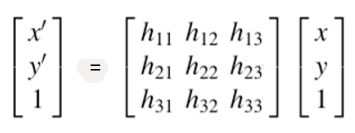
\includegraphics[width=4cm]{pHp.png}
    \caption{Breakdown of p' = Hp}
\end{figure}



\subsection{Rat Brain Atlas}
A rat brain atlas is representational map of the rat brain. Also, it shows where brain parts are ideally located even in areas that are difficult to find on stains. However, the atlases from Paxinos and Watson were digitally drawn by tracing the photographs of stains that they produced so it may not be perfect when finding exact measurements. Rather, it is best to continue using it and make good assumptions where brain pars are on a stain. 

\section{Prior Work}
Despite there has not been a product that specialize in visualizing rat brain parts on stains, there are current augmented reality (AR) programs that utilizes projective transformation mostly for occupational and or entertainment purposes. For instance, IKEA uses AR to help customers to visualize where they can place furniture before purchasing it. TikTok provides a platform for media creators to produce their own AR projects and send them around the world. 

What these products have in common to each other and to this project is the usage of projective image transformations. In addition, users may select a location or points on an object to project an image in that specific area. The rat brain atlas projection also currently requests users to select good matching points of where they want to find and visualize rat brain parts. 

\section{Methods}
\subsection{MATLAB}
MATLAB was used because it was easy to utilize for image processing and handling matrices. Also, it allowed image information to be accessed such as finding and manipulating an individual or a set of pixels. This was crucial because all pixels have several values (indices, color channels, gray scale intensity). Libraries and tools were included so that results were shown for work efficiently \cite{mat}. Primarily, it allows this project to use complex matrix operations to estimate and apply the homography transformation matrix. Also, MATLAB is efficient for program debugging especially when seeing specific result values that may mean faults in the algorithm. 

\subsection{Inputs}
\subsubsection{Images}
The program took an image of a rat brain stain and an image of the corresponding atlas. It was important to note that the stain and atlas must display the same measured coronal slice of the rat brain or else the output would be meaningless. A mismatch of the atlas and stain could cause brains parts to be mislabeled, researchers to feel confused, and the homography process to likely fail.

The images used for this project came from Paxinos and Watson's book of rat brain atlases and stains. One atlas of a coronal view of a rat brain and the corresponding acetylcholinesterase histochemistry (AChES) stain. The other corresponding stain is Timm-Nissl which is violet in color but more difficult for anyone to identify brain parts. While working on the project, the AChES stain was primarily used because brain parts and outlines were more noticeable. And, using that type of stain offered more confidence to people that were visualizing and giving feedback. 

Both images that were cropped to focus on a specific region led to better accuracy and meaning since less pixels are involved. And, focusing on one area makes selecting matching points more easier rather than choosing more points when matching larger images that have more brain parts.  

It is recommended that the image file type is JPEG format for the sake of its good compatibility with MATLAB. Some other image formats can be used but may require adding libraries to accommodate them. 

\subsubsection{Sets of Matching Points}
Selecting matching points from the atlas and the stain was a crucial make-or-break situation for homography to work. After resizing the atlas to be the same size as the stain, will be mentioned later, each pair must be carefully made so that the points are relatively close to each other if they were placed on the same image so that the estimated homography matrix would not cause extreme transformation and or the homography application to fail due to assigning pixels out of matrix index ranges. 

Both sets must have at least four points in order for the homography to be calculated. Adding more points can either improve the transformation to accurately map the brain parts or completely deteriorate the program run-time when applying the homography onto the atlas. In previous test cases, sets of five and six points were allowed to be used in situations of points of one image being not extremely distant from points. 

\subsection{Processing}
\subsubsection{Resizing image size}
The program automatically resize one image to be the same size of the other image reduce error when calculating and applying the estimated homography. Specifically, both images would have the same amount of pixels but one of them would be transformed. In the project, the atlas was resized in respect to the stain. 

\subsubsection{Estimating Homography Matrix}
First, the homography matrix must be found. Also, note that every homography matrix is different every time either set of pixel locations change because a matrix is created with specific pixel coordinates. From the p'~ Hp formula, equation AH ~ 0 was made to find H. The formula p' ~ Hp was rearranged to AH = 0:
\begin{figure}[htp]
    \centering
    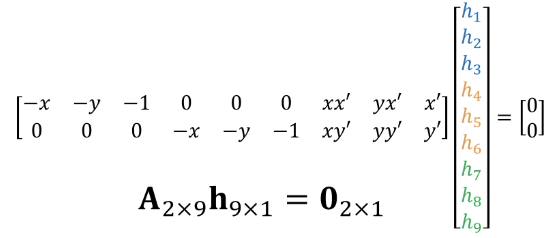
\includegraphics[width=6cm]{AH.png}
    \caption{Every h is a value in matrix H, x and y are pixel indices from the atlas, and x' and y' are pixel indices from the stain; This is matrix A with only one pair of pixels}
\end{figure}
The index values are placed into matrix A. Then, A was built represented all the pairs that were included in sets. 
\begin{figure}[htp]
    \centering
    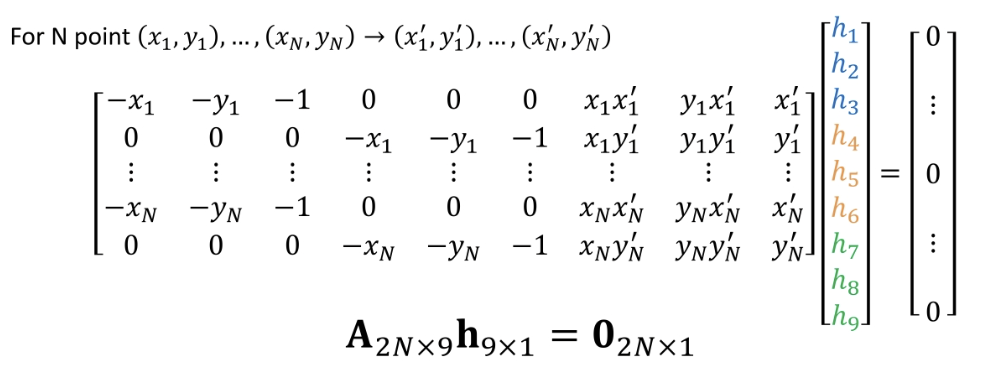
\includegraphics[width=8cm]{AN.png}
    \caption{Matrix A now has all N points}
\end{figure}
After building A, the values of h must be found so that resulting column vector should have all values of zero. However, realistically, finding values of h to get all values of the resulting column vector to be all zeroes were nearly impossible. So, the values of h were attempts to reach to zero. Closer to zeroes meant the better the solution and all points were well chosen.

From Ah = 0, A went through singular-value decomposition (SVD) to factorize for the best solution. This is a frequent encountered problem that is known as the homogeneous linear least squares problem, Ah = b. There are two solutions that can solve this general problem, but SVD only works because the h needs to cause A to equal or roughly close to 0. \cite{lect_B} The original form is SVD(A) which was calculated and resulted in three solutions: 


\begin{figure}[htp]
    \centering
    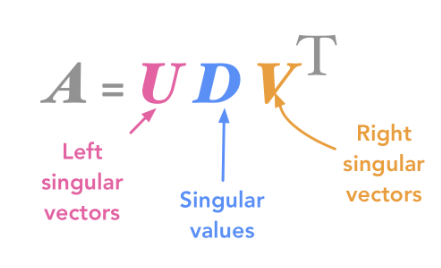
\includegraphics[width=6cm]{svd.png}
    \caption{UDV were resulting values after SVD(A)}
\end{figure}
The last vector in V was selected its values are relatively close to zero. And then, that vector is reshaped into a three-by-three matrix, which becomes the homography matrix.

\subsubsection{Transforming Rat Brain Atlas with Homography Matrix}
A blank canvas was made that is three times larger than the atlas because could be cases a pixel may be relocated outside of the original image boundary. At the start of iterating to create the transformed atlas, the initial indices were located the top left corner of the original image of that image was placed in the middle of the canvas. Next, every pixel of the original atlas image was relocated on the canvas. In other words, the homography matrix and pixel homogeneous coordinate operation was performed on all pixels of the atlas. Lastly, the canvas was cropped to the original size of the atlas.

\subsubsection{Filtering the Transformed Atlas}
Transformed atlases went through a transparency filter. This was possible because the alpha levels were accessible. An alpha level or value of an image determined the transparency such that values closer to one meant the image was less transparent and values closer to zero mean it was more transparent. Values around 0.35 were determined to be acceptable that the transparent transformed atlas overlay and the rat brain stain were visible and not hindering each other's view.

When the transparent transformed atlases were overlaid, most inner brain part outlines were barely noticeable. An edge canny filter, a MATLAB built-in filter that creates a black and white binary image, was applied onto a copy of a transformed atlas before changing the transparency of the it. The GitHub link to this project on the footnote of this page \footnote{https://github.com/hengjiaaan/fall23comps}

\subsection{Output}
At the end of the program, an image of rat brain stain with a transparent transformed atlas was displayed on the computer. A canny filtered transformed atlas was overlaid additionally as an option for user preference. Images were saved to compare with the the stain and the atlas separated. 

\section{Evaluation Metrics}
Because results are all visual and no technology was found to grade them, they are subjectively judged based on appearance. Accuracy was determined by matching noticeable brain parts on the stain. Furthermore, looking at the result causes one to think and feel how accurate the overlay is. Having this confidence with the help of the overlay was also considered because rat brain stains are already difficult to find parts that do not have visible outlines. Additionally, confidence could potentially affect a researcher's work afterwards such that it promotes one to have a good working and productive mindset. For instance, confidence and performance in sport athletes matter. More confidence leads to better performance and less confidence causes the opposite \cite{con}. Even though it is a small impact on work performance, confidence should still be considered since

What was be considered good was the following: high accuracy, clearness, confidence boosting, and short program run-time. For high accuracy, the atlas lines should provide a good estimate of where rat brain parts are located and should closely aligned with noticeable outlines of brain parts that were intended to be matched. Moreover, the atlas should be transformed in direct relation with the selected matching points so points from the atlas and the stain should be on top of or nearby each other in the image result. Next, the overlay must be clear such that it is not pixelated when the atlas was transformed.

This is determined by positive feedback, especially noting that the results provided a great visual-aid when visualizing where brain parts are located on the stain. Without it, a handful of people may have a difficult time visualizing where parts are located. Not everyone can visualize because each person has a different personality and mindset which affects this skill \cite{vis}. This fact also leads to an obstacle that some people may find when conducting experiments and analysis on rat brain stains in a learning environment. Feedback of noting this project's good worth is important to give

Lastly, the program should not take longer than a minute for to get matching points, calculating the homography matrix, transforming the atlas, and overlaying. This metric is mainly measured by the author/programmer since there is no front end and user friendly interface.

A result could be considered bad in contrary of the aspects mentioned above. The accuracy is poor if the atlas lines are extremely off-centered or not aligned with noticeable brain part outlines on a stain. When this is determined, the brain parts that are intended to be found on the stain are difficult to visualize. Also, the matching points are not overlapping each other in the overlay image. For confidence, one will feel skeptical toward the result. 

Metrics that determine how well homography was estimated was not used. The homography estimation and application is widely used and the implementation in this project was double checked multiple times to ensure that the calculations follow the estimation algorithm. What caused the homography to fail and miscalculated that led to an inaccurate and or an incomplete transformation was a poor selection of matching points. If the homography was judged, then homography matrices must produce the homogeneous linear least squares equation to be exactly zero for it to be considered good. However, this value from the equation can be greater than and close to zero which means the homography matrix produced is acceptable \cite{lect_y}.

To add on, if the homography matrix was being judged, then this metric decides how well the points were selected rather than the quality of the overlay. The points must be carefully selected because the homography matrix, determined by those points, changes the entire image of the entire atlas or a portion of the atlas. Additionally, the entire overlay will not transform or shape in the way that all atlas lines will perfectly align with the stain. Rather, the points chosen specify which area of the rat brain stain is being focused. That area and possibly some adjacent brain parts will have an accurate transformation but the overlay that are distant from the matching points will not be appropriately reshaped. 

Beyond the produced overlay images, another metric is considered which is the potential future work of this project. This is another subjective metric that is measured from others that can see how the project can be continued on. Also, it is relevant to the confidence metric that it can influence one's creativity and productivity. 

\section{Results}
\subsection{From The Author}
The homography transformation was applied on the entire atlas and a small portion of it. After numerous test trials were performed due to finding the best matching points, the overlay looks acceptable such that the atlas lines that were focused on were aligned with the stain. Fitting the entire atlas was not ideal besides to have it overlay based on the whole rat brain outline. However, this resulted in the inner parts were poorly transformed because the transformation was not made for them. 

\begin{figure}[htp]
    \centering
    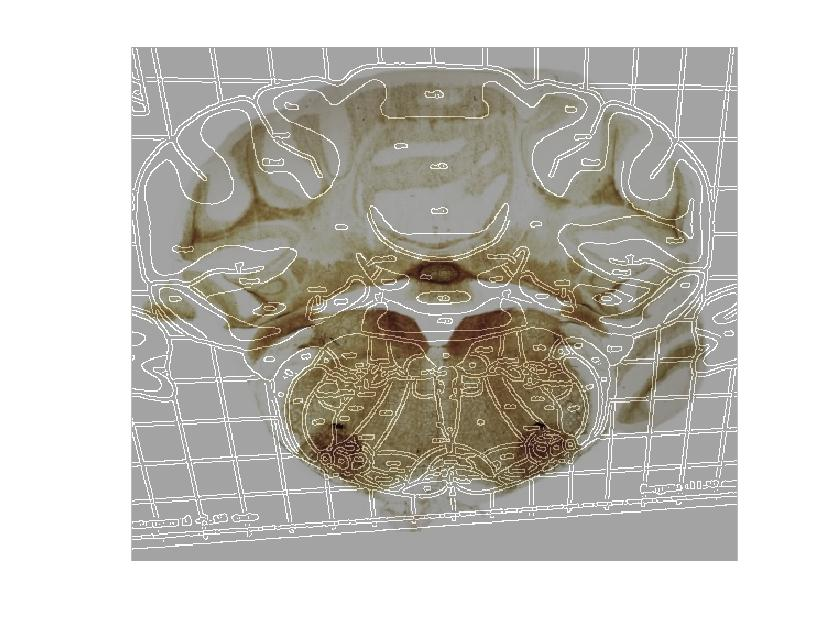
\includegraphics[width=7cm]{result_e.jpg}
    \caption{Canny filtered overlay on entire rat brain stain, six matching points used}
\end{figure}

At this point, the results were not great and meaningless since the accuracy was super poor. Even if adding more matching points were to happen in estimating the homography, the transformation would still be unacceptable. However, homography did well on small areas of the rat brain stain. The overlay that focused on the facial nucleus looked accurate and could raise the confidence in neuroscience researchers and students. The atlas lines were roughly aligned with the stain but it was not perfect so that the atlas lines were exactly on top of brain part outlines. 

Both images of the atlas and the stain were zoomed in screenshots from the original Paxinos and Watson's digital book. Those were used instead of cropping the images of the entire atlas and stain because doing so causes the image to look blurry. Blurry images could have been filtered with a sharpening filter to make atlas and stain lines more prominent but the visually unacceptable since some original details in the stain are lost. Pre-cropped images were better because they were more clear before and after transformation and overlay. 
\begin{figure}[htp]
    \centering
    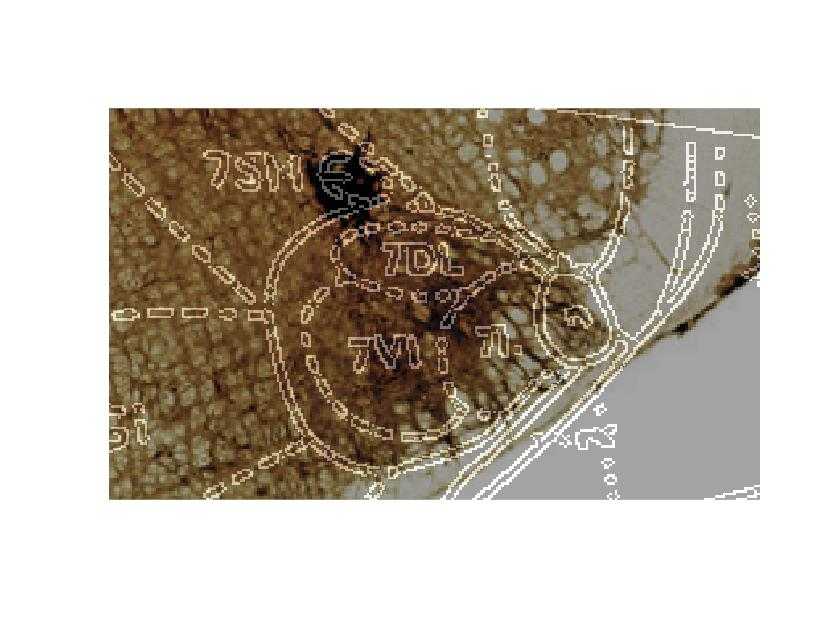
\includegraphics[width=7cm]{result.jpg}
    \caption{Canny filtered overlay on the lower rat brain stain, parts of the facial nucleus}
\end{figure}

\subsection{Professional and Student Feedback}
Professional feedback was given by Professor Kevin Urstadt from the cognitive science department. The image of the entire stain overlay (Figure 5) was shared with him first weeks before completing this project. He mentioned it was a good starting point but the accuracy for many parts inside the rat brain was poor. Following up, the most up to date progress (Figure 6) was presented to shift focus toward transforming a small portion of the atlas. Professor Urstadt noted that this progress was a significant improvement on the accuracy. Also, he thought it was more meaningful to analyze one area or brain part at a time since the homography matrix could not handle multiple parts simultaneously. Professor Urstadt liked the aspect of having a visual-aid map at a very quick turnaround time since lab experiments without this would take hours to complete. 

The two options of the unfiltered and canny filtered overlays were helpful for his students that have various amounts of neuroscience knowledge. Professor Urstadt mentioned the unfiltered overlay would be great for beginners since it showed parts with different colors for each one. The canny filtered overlay could be used for those have sufficient experience with rat brain stains and atlases since the filter makes the edges and lines of the outline to show prominent white while the spaces in between are black or dark after the alpha levels were decreased.

The clearness of the atlas was still subjective matter that was progressively worked on during the process on the project. It was because the overlay alpha level, the transparency, causes the resulting image visuals to look unpleasing. Professor Urstadt was not satisfied with the unfiltered overlay if the alpha levels are too high which causes the the atlas to be show more prominently. The light blue areas from the rat brain parts within the atlas created an opaque greyish color that also made the stain look cloudy. Also, there were other fiber-like lines within those parts so it was noted that those should be preserved too. When the alpha levels were reduced more, the stain could be seen better in both unfiltered and filtered options but another drawback comes into play of having a visually appealing atlas. Specifically, Professor Urstadt was more satisfied when the alpha level was around 0.35 for both options which shows a more transparent atlas. Because there is no one-value-fits-all, the clearness could be maximized if the Professor Urstadt or any researcher have the ability to adjust the alpha levels to their liking.

Furthermore, he felt confident that future work could happen that goes beyond image processing and reach larger goals (mentioned in future work and discussion).
 
 Informal feedback was given at the senior comprehensive project showcase. At the time, two types of results were shown to the audience. One displayed the overlay on the entire stain (Figure 5) and the other displayed the overlay on the small stain area (Figure 6). Students with a background in cognitive and neuroscience sciences were fascinated with the results. A most frequent key point was how the overlay was super helpful to visualize the stain with and without the overlay. Another was the program could have reduced the lab time and accelerated the learning curve if it was accessible to them. 
 
 Students that had little to no cognitive science and neuroscience background understood the meaning of the transformed atlas. They also thought it was helpful if they were to take a course in neuroscience without having knowledge in the subject. And, it was a good glimpse of some work that neuroscience students do if looking into taking a class in the future. 

 Clearness aspect was catered to individual preferences. A few examples of overlays with different alpha values were presented to students and there was a mix of choices which alpha value they desired. But, because the level of transparency was selectable, every student noted the image result of their transparency choice was nicely shown. 

\section{Ethical Considerations}
Because this project primarily uses homography, it is biased that only one solution was used to perform projective image transformation. There were other libraries and built-in functions that demonstrate the transformation; however, most of them do not allow access to the values being produced and how they were selected or made during the calculations. Without using short-cut functions, the implementation of homography is great what and where it failed in the process.

Another argument was using basic reshaping or re-scaling the atlas parts based on the distances of x coordinates and the distances of y coordinates could have been the more direct and easier solution. But, there are a few problems with this. First, the reshaping of the atlas parts would cause everything in the atlas to change too. This method only required one pair of matching points. Adding more pairs would cause the transforming of all pixels to iterate multiple times which homography does not do. Homography reshapes the atlas in one iteration of transforming all the pixels. In other words, the homography matrix, a three by three matrix, transforms the pixels in relation with at least four pairs of matching points. This also means that the transformation is meaningful and has some direct relationship with the selected matching points \cite{lect_y}. In contrast, the basic scalar reshaping means only one pair of matching points for every iterative transformation that occurs. 

The use of the stains and the atlases were sourced from Paxinos and Watson but they are copyrighted material. Because of this, the use of stains and atlases could not be utilized if this project is available to create images for public and or publishing use. Thus, images must be sourced else where. The solution to this is to make personal photographs and atlases of rat brain sections or find an open source that have relevant images since homography mainly focuses on transformation of selected points rather than points chosen by a well-taught machine that could only work with rat brain stains and atlases that must have specific visual qualities.

Furthermore, possibilities of not having access to high quality images of stains and atlases could not solved. Because of the lack of sources, the capability to shorten lab time and work would be nonexistent and the use of the program would be ineffective.


\section{Future Work and Discussion}
This project is a good stepping stone toward a higher goal; however, furthering the project to be more accurate, efficient, and convenient requires work to be done in different branches of computer visions. Some could have been accomplished or were achievable however time and the lack of little to no knowledge of other branches such as using convolutional neural networks and detecting specific object features caused the project to be mostly focused on homography transformation. But the following work could be accomplished so that it becomes an additional component to create a larger project in the long run. 

\subsection{Mosaic of Transformed Overlays}
Even though using homography transformation was impossible to perform on the entire atlas, transforming individual small areas and stitching them together using homography and traditional mosaic stitching could be a more efficient way to create a more accurate transformed atlas. Mosaic stitching is commonly used to create a panoramic image by stitching two or multiple images together based matching features of objects shown in them \cite{Abbadi_2021}. 

\subsection{Automating Matching Points, Feature Matching Detection}
Having an automated matching system would reduce stress and time compared to repetitively manually finding and inputting matching points that have various homography transformation results. Already, this project lacks this which not ideal if it was supposedly needed to reach a higher goal of a quick and convenient automated system. 

A new feature matching detection system could significantly help. It is one of the main aspects in computer vision but is not image processing based. MATLAB has a built-in function that matches features between two images of the exact object. Moreover, it attempts to find the perfect point that is exactly the same on both images \cite{lowe}. But, because the project tries to match two different objects, a new system must be implemented so that brain features are identifiable and must make a match between the stain and the atlas. This is a more large scale project; moreover, creating data sets might be required for machine learning purposes.

\subsection{Live Camera Projective Atlas, Augmented Reality Application}
Like creative media applications, a program that transforms and projects on live camera would be an ultimate goal. It would require perfecting the atlas fitting, creating a new feature detection program, and other software to make this happen. In addition, a powerful camera that could zoom onto a stain like a microscope would be necessary so it can be connected to one unit that controls the entire program. 

\section{Replication Instructions and Code Architecture Over}
Before downloading the files necessary for the program to run, MATLAB must be installed first. No additional libraries are required. After appropriately installing MATLAB, the files in the GitHub repository can be downloaded and placed in a single folder. If MATLAB was already installed and been used with other files, create a separate folder that only contains the files for the program since MATLAB cares about which directory/folder wants to be used. 

The main file is comps\_main.m which will be primarily used to run the program. Other files are mostly functions and images that will be used in the main file. The MATLAB files can be thought of scripts with lines that can be individually copied and executed into the command line. It is recommended that a user should execute one line at a time because executing multiple lines may cause the program to malfunction and or stop due to user error and pop-up interactive windows may not appear because the script shows a display multiple times if the entire script is executed. Executing one or multiple lines executively in a script can be done by left-click dragging the cursor over the entire line(s) and execute the F9 button. This is the typical method that worked on this project but other solutions can be found on the MATLAB online documentation. 

The used images are provided in the repository. Other images outside the repository can be personally used but do not add them to the remote repository. 

Other notes
\begin{itemize}
\item Manually choose matching points between the stain and the atlas. Mismatching them or selecting points that are distant to points from the other image will cause the homography transformation to fail
\item There is a pre-cropped stain and atlas. Creating other cropped stains and atlases can be done which is available in the main file. However, doing so will result in lower quality, pixelated, and or blurry images.
\end{itemize}

The code architecture of the main script is the following:
\begin{figure}[htp]
    \centering
    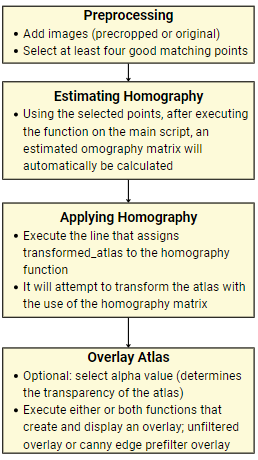
\includegraphics[width=8cm]{overview.png}
    \caption{comps\_main.m architecture overview}
\end{figure}


More details about individual functions and algorithms can be seen in the files/scripts in the GitHub repository. Some lines of code is straightforward and no additional comments are necessary to explain \footnote{https://github.com/hengjiaaan/fall23comps/tree/main/matlab\_files}.

\printbibliography
\end{document}

\printbibliography
\end{document}
